\documentclass[12pt, letterpaper]{article} 

\usepackage{amsmath, amssymb, amsthm, enumerate, graphicx}

\title{MATH 114 HW 4}
\author{Dani Nguyen}
\date{Winter 2025}

\begin{document}
\maketitle
\graphicspath{ {./} }

\noindent \textbf{Question 1}
\begin{enumerate}[a.]
    \item Define $\bar X = \frac 1n \sum_{i=1}^{n}X_i$ and 
    $\mathbb{E}(X) = \pi \text{ since } X_0 \sim \pi, X_i \sim \pi\ \forall i$. We have
    \begin{align*}
        \mathbb{E}(\bar X) &= \mathbb{E}\left(\frac 1n \sum_{i=1}^{n}X_i\right) \\
        &= \frac 1n \sum_{i=1}^{n}\mathbb{E}(X_i) \\
        &= \frac 1n \cdot n \mathbb{E}(X) \\
        &= \mu
    \end{align*}
    \item We have $\mathbb{P}(X_{t+s} = j, X_t = i)=\mathbb{P}(X_{t+s = j | X_t = i})\mathbb{P}(X_t = i)$
    \begin{align*}
        \mathbb{E}(X_tX_{t+s}) &= \sum_{i,j = 1}^{N} (ij) \mathbb{P}(X_{t+s} = j, X_t = i) \\
        &= \sum_{i,j = 1}^{N} (ij) \mathbb{P}(X_{t+s} = j | X_t = i) \mathbb{P}(X_t =i) \\
        &= \sum_{i,j = 1}^{N} (ij) (P_{ij})^s \cdot \pi(i) \\
        &= \sum_{i,j = 1}^{N} (ij) \mathbb{P}(X_{0+s} = j | X_0 = i) \mathbb{P}(X_0 = i) \\
        &= \sum_{i,j = 1}^{N} (ij) \mathbb{P}(X_s = j, X_0 = i) \\
        &= \mathbb{E}(X_0X_s)
    \end{align*}
    \item $\text{Var}\bar X \ne \frac 1n \text{Var}X$ because $X_i$ depends on $X_{i-1}$, therefore
    they are not independent, and we can not compute the sum $\sum_{i=1}^{n}\text{Var}X_i$.
\end{enumerate}
\newpage
\noindent \textbf{Question 2} \\
\begin{enumerate}[a.]
    \item \begin{enumerate}[i.]
        \item \ \\ 
        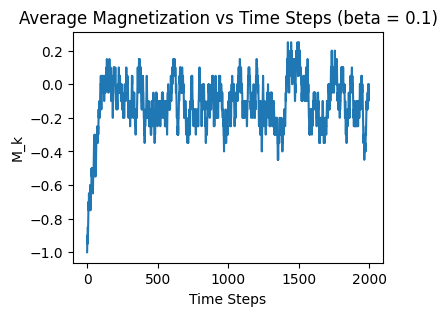
\includegraphics{2aibeta0.1.png} \\
        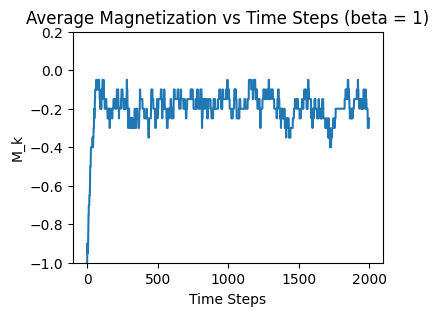
\includegraphics{2aibeta1.png} \\
        
\includegraphics{2aibeta5.png} \\
        Note that 
        \begin{align*}
            \alpha = \frac{f(W)}{f(X_i)} = \frac{\exp(-\beta H(W))}{\exp(-\beta H(X_i))} = \exp(-\beta(H(W)-H(X_i)))
        \end{align*}
        Therefore the bigger the $\beta$, the lower $\alpha$
        
        \item 
    \end{enumerate}
\end{enumerate}

\noindent \textbf{Question 3} \\

\end{document}